% ---------------------------------------------------------------------------
% Author guideline and sample document for EG publication using LaTeX2e input
% D.Fellner, v1.13, Jul 31, 2008

\documentclass{egpubl}
\usepackage{eurovis2019}

% --- for  Annual CONFERENCE
% \ConferenceSubmission   % uncomment for Conference submission
% \ConferencePaper        % uncomment for (final) Conference Paper
% \STAR                   % uncomment for STAR contribution
% \Tutorial               % uncomment for Tutorial contribution
% \ShortPresentation      % uncomment for (final) Short Conference Presentation
% \Areas                  % uncomment for Areas contribution
% \MedicalPrize           % uncomment for Medical Prize contribution
% \Education              % uncomment for Education contribution
% \Poster                 % uncomment for Poster contribution
% \DC                     % uncomment for Doctoral Consortium
%
% --- for  CGF Journal
% \JournalSubmission    % uncomment for submission to Computer Graphics Forum
% \JournalPaper         % uncomment for final version of Journal Paper
%
% --- for  CGF Journal: special issue
% \SpecialIssueSubmission    % uncomment for submission to , special issue
% \SpecialIssuePaper         % uncomment for final version of Computer Graphics Forum, special issue
%                          % EuroVis, SGP, Rendering, PG
% --- for  EG Workshop Proceedings
% \WsSubmission      % uncomment for submission to EG Workshop
% \WsPaper           % uncomment for final version of EG Workshop contribution
% \WsSubmissionJoint % for joint events, for example ICAT-EGVE
% \WsPaperJoint      % for joint events, for example ICAT-EGVE
% \Expressive        % for SBIM, CAe, NPAR
% \DigitalHeritagePaper
% \PaperL2P          % for events EG only asks for License to Publish

% --- for EuroVis 
% for full papers use \SpecialIssuePaper
% \STAREurovis   % for EuroVis additional material 
\EuroVisPoster % for EuroVis additional material 
% \EuroVisShort  % for EuroVis additional material

 \electronicVersion % can be used both for the printed and electronic version

% !! *please* don't change anything above
% !! unless you REALLY know what you are doing
% ------------------------------------------------------------------------

% for including postscript figures
% mind: package option 'draft' will replace PS figure by a filename within a frame
\ifpdf \usepackage[pdftex]{graphicx} \pdfcompresslevel=9
\else \usepackage[dvips]{graphicx} \fi

\PrintedOrElectronic

% prepare for electronic version of your document
\usepackage{t1enc,dfadobe}

\usepackage{egweblnk}
\usepackage{cite}

% For backwards compatibility to old LaTeX type font selection.
% Uncomment if your document adheres to LaTeX2e recommendations.
% \let\rm=\rmfamily    \let\sf=\sffamily    \let\tt=\ttfamily
% \let\it=\itshape     \let\sl=\slshape     \let\sc=\scshape
% \let\bf=\bfseries

% end of prologue
% ---------------------------------------------------------------------
% EG author guidelines plus sample file for EG publication using LaTeX2e input
% D.Fellner, v2.02, Jan 25, 2017


\title[Improving the Scalability of Interactive Visualization Systems for Exploring Threaded Conversations]%
      {Improving the Scalability of Interactive Visualization Systems for Exploring Threaded Conversations}

% for anonymous conference submission please enter your SUBMISSION ID
% instead of the author's name (and leave the affiliation blank) !!
% for final version: please provide your *own* ORCID in the brackets following \orcid; see https://orcid.org/ for more details.
\author[A. McNutt \& G. Kindlmann]
{\parbox{\textwidth}{\centering A. McNutt and G. Kindlmann
%        S. Spencer$^2$\thanks{Chairman Siggraph Publications Board}  
        }
        \\
% For Computer Graphics Forum: Please use the abbreviation of your first name.
{\parbox{\textwidth}{\centering Department of Computer Science, University of Chicago
%        $^2$ Another Department to illustrate the use in papers from authors
%             with different affiliations
       } 
}
}
% ------------------------------------------------------------------------

% if the Editors-in-Chief have given you the data, you may uncomment
% the following five lines and insert it here
%
% \volume{36}   % the volume in which the issue will be published;
% \issue{1}     % the issue number of the publication
% \pStartPage{1}      % set starting page


%-------------------------------------------------------------------------
\begin{document}

\teaser{
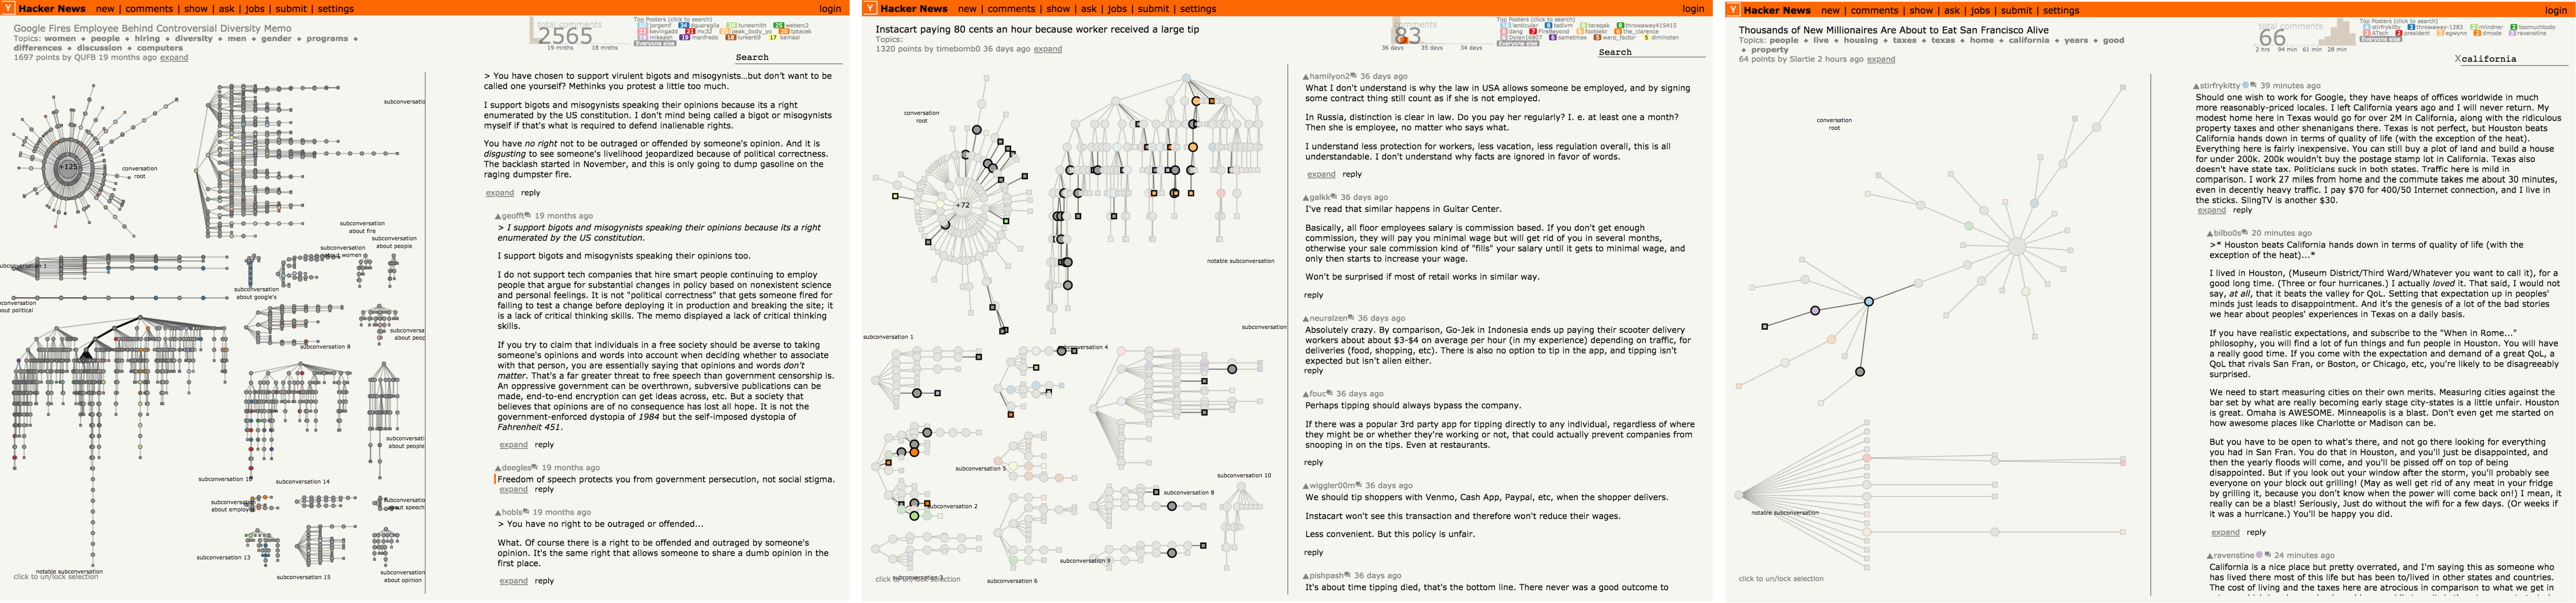
\includegraphics[width=\linewidth]{images/teaser.pdf}
\centering
\caption{
Three HackerNews conversations rendered using ForumExplorer.
%
In the left image the user has moused over a particular sub-conversation, in the center they have scrubbed to a point in time, and in the right they have searched for a particular topic tag.
}
\label{fig:teaser}
}

\maketitle
%-------------------------------------------------------------------------
\begin{abstract}
Large threaded conversations, such as those found on YCombinator's HackerNews, are often rendered in a manner that presents individual comments clearly but can obscure larger trends or patterns within the conversational corpus.
%
Previous works have addressed this problem through graphical-overviews and NLP-generated summaries.
%
These efforts have generally been designed around an ideal size of data, which can be difficult to use for large or deeply-nested conversations, and have sometimes require non-trivial offline processing time, which makes them impractical for day to day usage.
%
We refine these approaches through the construction of a Chrome Extension, Forum Explorer, that expands prior art through a collection of novel design strategies that enable this type of representation to handle wider ranges of data in real time.
  \\
%   Leave one blank line after the abstract, 
%   then add the subject categories according to the ACM Classification Index 
%-------------------------------------------------------------------------
%  ACM CCS 1998
%  (see http://www.acm.org/about/class/1998)
% \begin{classification} % according to http:http://www.acm.org/about/class/1998
% \CCScat{Computer Graphics}{I.3.3}{Picture/Image Generation}{Line and curve generation}
% \end{classification}
%-------------------------------------------------------------------------
%  ACM CCS 2012
%   (see http://www.acm.org/about/class/class/2012)
%The tool at \url{http://dl.acm.org/ccs.cfm} can be used to generate
% CCS codes.
%Example:
\begin{CCSXML}
<ccs2012>
<concept>
<concept_id>10010147.10010371.10010352.10010381</concept_id>
<concept_desc>Human-centered computing~User interface design</concept_desc>
<concept_significance>300</concept_significance>
</concept>
<concept>
<concept_id>10010583.10010588.10010559</concept_id>
<concept_desc>Human-centered computing~Visualization</concept_desc>
<concept_significance>200</concept_significance>
</concept>
<concept>
<concept_id>10010583.10010584.10010587</concept_id>
<concept_desc>Human-centered computing~Graph drawings</concept_desc>
<concept_significance>100</concept_significance>
</concept>
</ccs2012>
\end{CCSXML}

\ccsdesc[300]{Human-centered computing~User interface design}
\ccsdesc[200]{Human-centered computing~Visualization}
\ccsdesc[100]{Human-centered computing~Graph drawings}


\printccsdesc   
\end{abstract}





%-------------------------------------------------------------------------
\section{Introduction}


%%%
%%% Figure 1
%%%
\begin{figure}[htb]
\centering
% the following command controls the width of the embedded PS file
% (relative to the width of the current column)
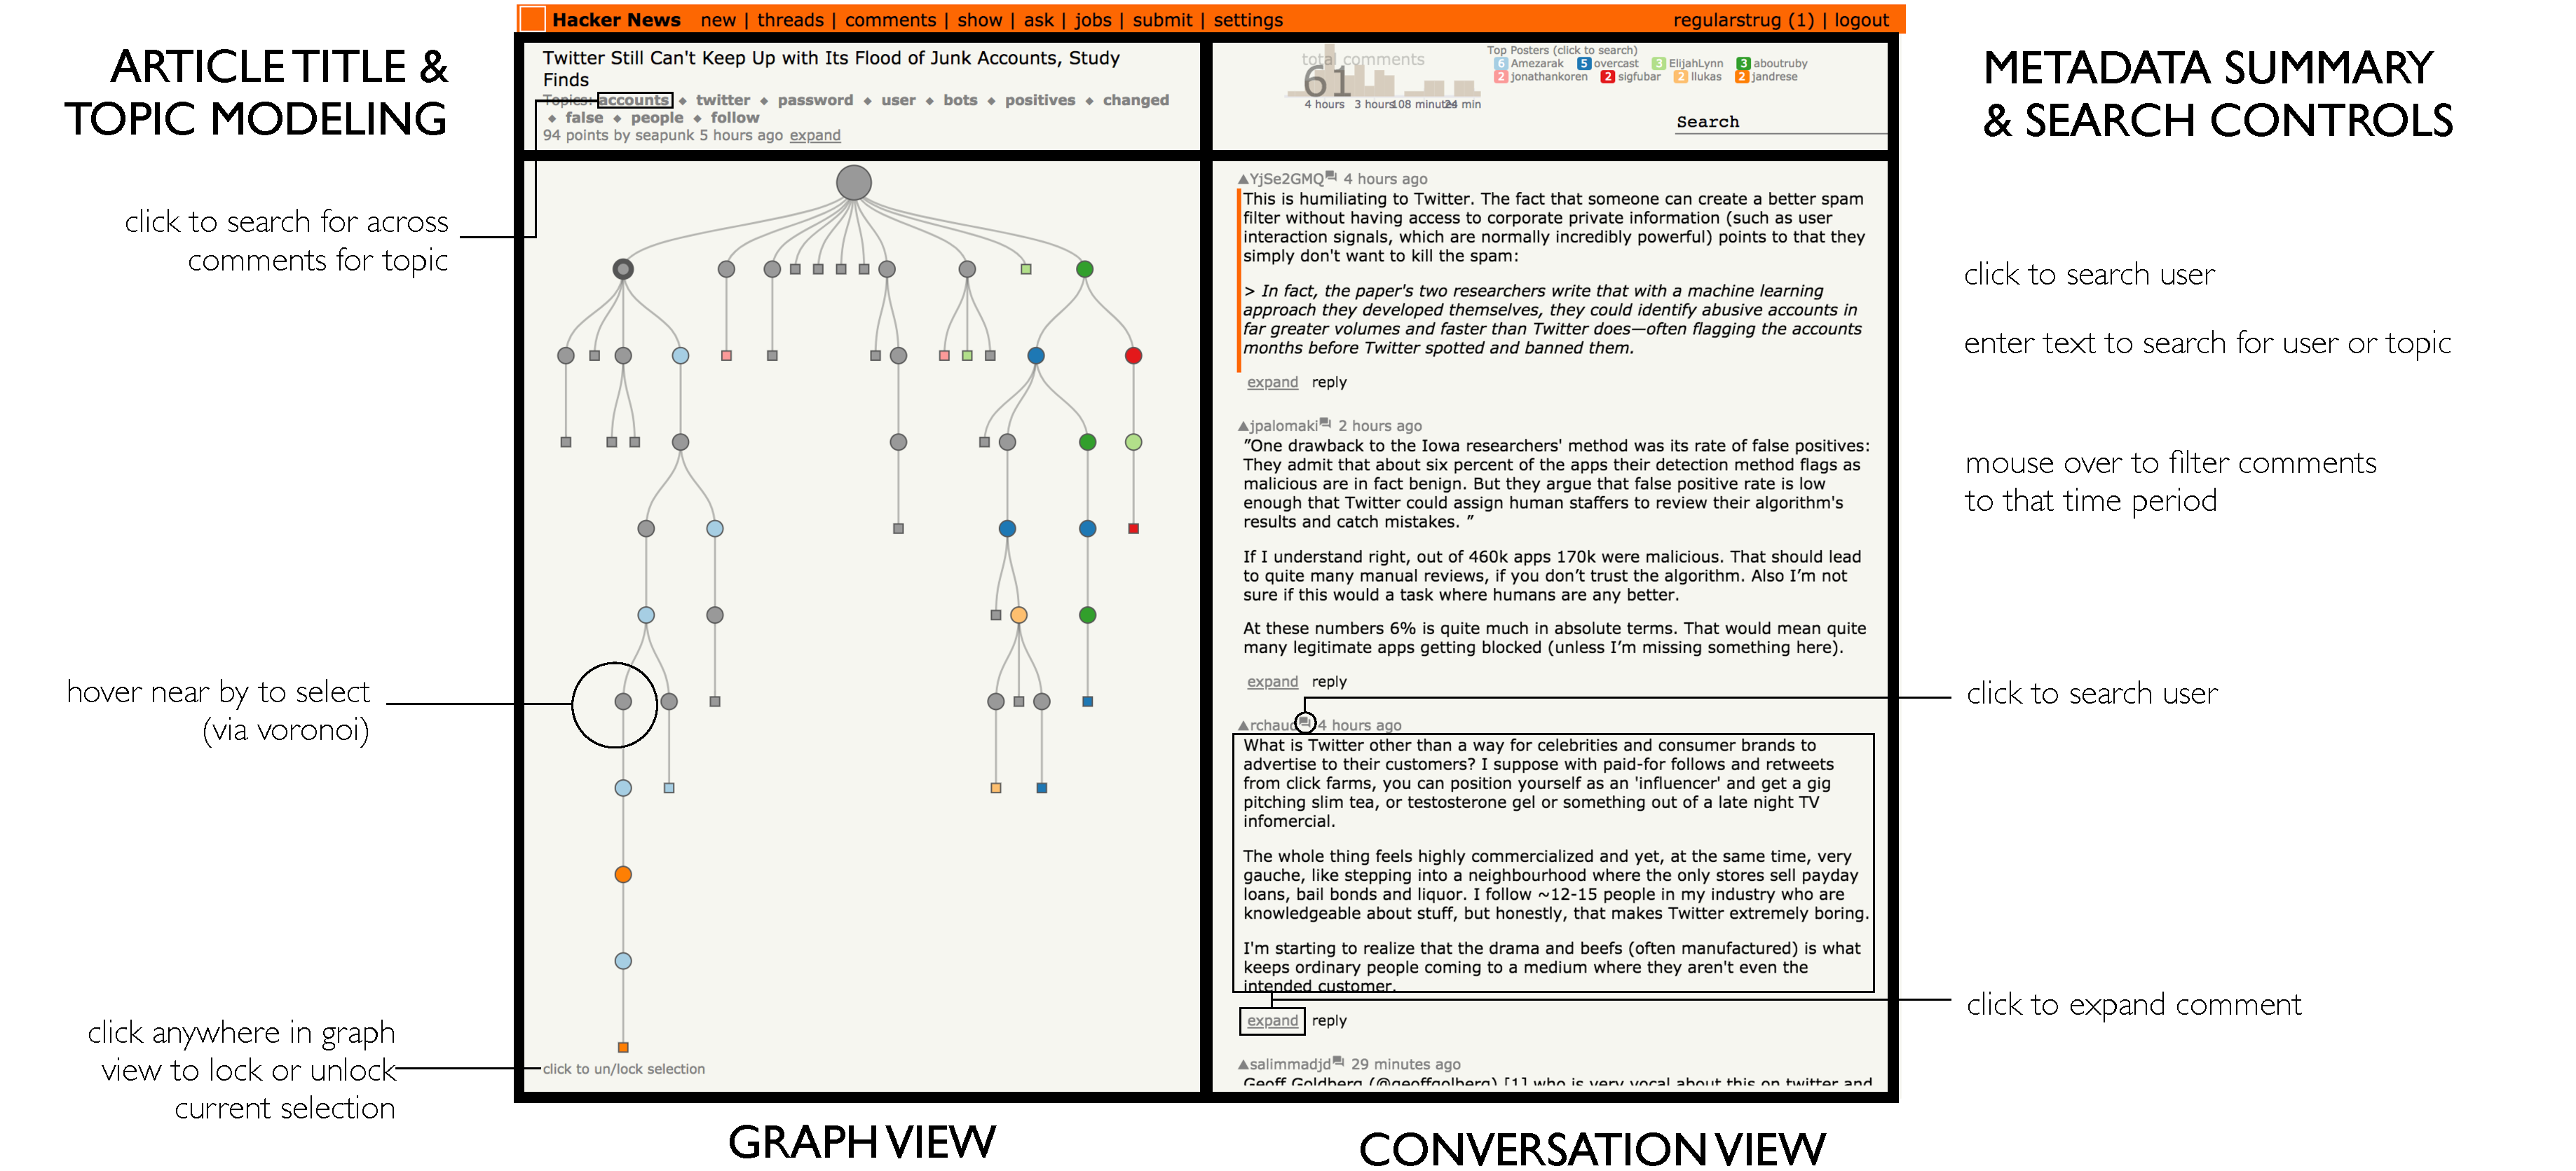
\includegraphics[width=0.9\linewidth]{images/explainer.pdf}
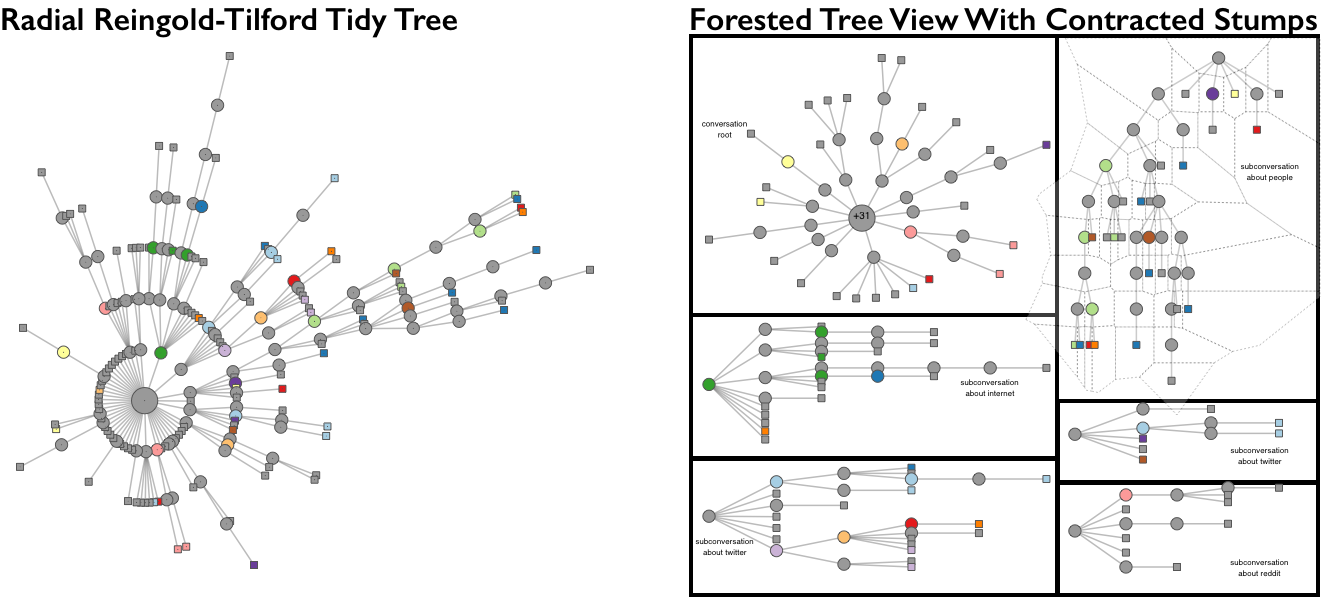
\includegraphics[width=0.9\linewidth]{images/forested-tree-view-example.pdf}
% replacing the above command with the one below will explicitly set
% the bounding box of the PS figure to the rectangle (xl,yl),(xh,yh).
% It will also prevent LaTeX from reading the PS file to determine
% the bounding box (i.e., it will speed up the compilation process)
% \includegraphics[width=.95\linewidth, bb=39 696 126 756]{sampleFig}
%
%  \parbox[t]{.9\columnwidth}{\relax
%          For all figures please keep in mind that you \textbf{must not}
%         use images with transparent background! 
%         }
%
\caption{
\label{fig:explainer}
Annotated view explaining the components of the UI (top) and a visual explanation of Forested Tree Layout (bottom). 
}
\end{figure}


Conversation on the internet takes many shapes and forms. 
%
Of particular interest are asynchronous threaded conversations, such as those found reddit, in which users comment on the root of the conversation or on any previous comments, thus forming a tree. 
%
Unfortunately the design of these digital spaces typically do not allow for users to interact with the conversational corpus as a whole, which can limit or impede understanding of the community opinions and insights about a topic.
%
Further, participants in these conversations might provide domain expertise or other valuable insights, which can get lost in the crowd.
%
These sorts of analytic expertise-seeking tasks are sometimes the primary motivators for this type of forum usage \cite{barik2015heart, hoque2014convis}, which manifest themselves as discover and browse tasks in the visualization task typology \cite{brehmer2013multi}.



Previous works have developed a fascinating collection of UI paradigms to augment and enhance forums in this space. 
%
A common trend among them features an overview of the conversational thread encoded as a graph-like structure, which the user then interacts with in a details-on-demand \cite{shneiderman1996eyes} and scented-widget-like \cite{willett2007scented} patterns to expose components of the discourse (such as groups or chains of comments). 
%
% The first work of this type is Donath et al's Loom, which introduced the idea of graphical exploration of comment graphs \cite{donath1999visualizing}. 
 %
 Early work addressing this includes Donath et al's \textbf{Loom}, which introduced the idea of graphical exploration of comment graphs \cite{donath1999visualizing}, and Sack's \textbf{Conversation Map}, which represented conversation as a tree-like structure \cite{sack2000conversation}. 
 %
 Wattenberg et al introduced a split pane view, one pane providing a graphical overview (which mirrors the multiply-indented form that threaded conversation are usually depicted in) and the other displaying currently selected comments \cite{wattenberg2003conversation, dave2004flash}.
% 
Pascual-Cid et al later introduced a space filling radial tree layout \cite{pascual2009exploring}. 
%
Narayan et al construct \textbf{tldr} which focuses on reddit and encodes the conversation as an icicle diagram \cite{narayan2010not}. 
%
Butler puts these ideas in practice through a Chrome Extension, \textbf{Treeverse}, that visualizes the conversation trees on Twitter \cite{treeverse}.
%
Hoque et al break from purely metadata visualization by adding topic modeling and sentiment analysis  \cite{hoque2014convis, hoque2016interactive}.
%
While these tools are uniformly well received by their evaluation audiences, they have failed to gain widespread usage.
%
This may be because visualization based overview systems are not well aligned with the types of tasks that people pursue on threaded forums, a problem which remains unclear from the previous works.
%
While this issue remains prescient, we are unable to directly address it in the scope of this work.
%
Instead we assert that that previous iterations may have failed to gain traction because they do not possess accessible or online implementations, force their users out of their usual environment, and are designed around a single ideal size of conversation and thus become cumbersome or difficult to use when conversations of interest fall outside of that target domain.






\section{Forum Explorer}

We address these problems through \textbf{Forum Explorer}, a Chrome Extension that repurposes the layout of yCombinator's social news website, HackerNews \cite{hackernews}, to facilitate better data exploration.
%
We focus on HackerNews because it has an active community with more than 8.5 million comments that often have a highly nested structure and is seen as a reputable source of domain-expert opinions \cite{barik2015heart}.
%
Our implementation captures many of the features from prior art, including a tree based graphical overview, that denotes comments as vertices and parentage as edges, and NLP-based summaries.
%
We further detail our design in Figure \ref{fig:explainer} (top). 
%
This design emphasizes the discovery of sub-conversations as a mechanism for exploration.
%
We provide topic-summaries of the conversation corpus through the use of Latent Dirichlet Allocation (via lda.js \cite{lda-js}), which we compute on a caching micro-service hosted on Heroku. 



Our design is derived from two observations about the behavior of our domain of focus.
%
\textbf{Firstly}, we observe that the weights of rooted branches tends to be heavily dominated by a small collection of sub-trees.
%
To this end, we introduce a novel Forested Tree View which splits threaded conversations into a collection of smaller and more legible trees, see Figure \ref{fig:explainer} (bottom).
%
We prune the heaviest branches from the root and present them as independent trees, which we arrange in space by computing a treemap layout.
%
This technique allots each subtree an appropriate amount of screen area for the number of comment nodes that it contains and provides a helpful responsiveness for the layout.
%
We render the root as a radial tree in order to give it visual significance, and the rest of the subtrees as linear Reingold-Tilford tidy trees whose direction (left-right vs up-down) are aligned with the longer container dimension.
%
This approach allows for ample visual space to provide in-situ annotations and textual guides. 
%
We find empty space in the graphic to add annotations (which are single topic summaries for that subtree) by constructing a Voronoi for the complete layout, and then finding the largest (and hence emptiest) cell for each subtree.
%
\textbf{Secondly}, we observe that large conversations tend to be have a large number of rooted stumps that add substantial visual noise.
%
We address this by collapsing these stumps into the root and adding a textual annotation to the root indicating their presence, which allows the user to still interact with them via our details on demand pattern.
%
\textbf{Together} these features provide the user a rich set of overview tools that directly facilitate both browse and  tasks \cite{brehmer2013multi}.
%
Our implementation visually scales well and maintains responsiveness up to the largest available HackerNews thread \cite{hackernews-biggest}, as in Figure~\ref{fig:teaser}.





%-------------------------------------------------------------------------
\section{Conclusions \& Future Work}
We have presented \textbf{Forum Explorer}, a tool for exploring threaded conversations on HackerNews. 
%
Our primary contribution is a novel graph layout that facilitates better scalability in exploring threaded conversations, however we believe that there is room for our tool to make further useful contributions.
%
Unfortunately, it remains unclear whether or not this type of application has long-term utility (as opposed to novelty-driven laboratory results).
% \cite{isenberg2013systematic}).
%
%The best evidence of substantive usefulness is that Treeverse is (in addition to being modestly popular, cf. its 2400 active users) used by Rao et al to study the way that domain specific knowledge expressed on twitter becomes deeply siloed \cite{twittercanoes}.
%
%Rao et al's study, which makes use of \textbf{Treeverse}, of the way in which domain specific knowledge expressed on twitter becomes deeply siloed suggests that there may in fact be substantive usefulness for this type of system, but it remains unclear\cite{twittercanoes}.
%
Rao et al's study (which uses \textbf{Treeverse}) of the way in which domain specific knowledge expressed on twitter becomes siloed suggests that this type of system may have genuine utility \cite{twittercanoes}.
%
%
The practical usability of our application makes it well positioned to conduct a longitudinal study that could answer questions about the effectiveness of task completion in realistic user settings.
%
While all work in this vein has targeted the desktop, future work might consider how these design strategies can be translated to mobile environments.
%
Finally we believe the design strategies expressed in this work could also have applicability to systems outside of threaded conversations, such as visualizations of the scholarly citation graph.



% While these studies usefully demonstrate the usability of the structural design elements in general, their context as laboratory based analyses precludes them from providing longitudinal information about the way users might interact with this type of tool when they are able to incorporate it into their day to day workflow. Forum Explorer is well positioned 

% Our current design process has, in the lens of data feminism, been unfeminist. Our design process happened without consultation of those who might find the application (other than perhaps ourselves). While we are able to rest on the many of the observations from ConVis's prior user studies in the topic, individual forum users tend to have individual expectations about their tools.

% The specific utility of this type of conversation overview tool remains unclear, the lessons learned from ours and other systems could readily be applied to graph analysis problems of a similar size and scale. Analysis of locally relevant articles in the scholarship graph are one such example of this type of system.




%-------------------------------------------------------------------------

%\bibliographystyle{eg-alpha}
\bibliographystyle{eg-alpha-doi}

\bibliography{forum-bib}

\end{document}

